% !TeX root = ../thuthesis-example.tex

\begin{survey}
\label{cha:survey}

\title{PMT Iterative Calibration}
\maketitle


\tableofcontents

\section{Introduction}

Photomultiplier tubes (PMTs) with microchannel plate (MCP) and atomic layer deposition (ALD) has been applied in 
Jiangmen Underground Neutrino Observatory (JUNO) and China Jinping Underground Laboratory (CJPL)\cite{Chen2023Nov}.
It's proposed to overcome the poor time performance of the existing dynode MCP-PMT, 
aiming to increase the quantum effeciency of photoelectrons (PE). Lin Chen et al concluded from Monte Carlo simulation 
that 97.5\% of photoelectrons land on the MCP active area, emitting multiple secondary electrons from ALD.
The acceptance fraction of impinging PE is nearly 100\%\cite{Chen2023Nov}.

However, these MCP-PMTs possess a unique long tail structure in their charge response spectrum
compared to traditional dynode PMTs, from which calibration difficulty arises\cite{Zhang2023Oct}.
Traditionally, dynode PMTs' single electron response (SER) charge spectrum resembles Gaussian or Poisson distribution.
Therefore, a Tweedie distribution would be enough to calibrate the charge response expectation $\mu_q$ and variance $\sigma_q^2$.

For now, some papers on ALD MCP-PMTs are published.
For 8-inch MCP-PMTs with ALD, Aiqiang Zhang et al only fitted local peak by Gaussian model,
but didn't calibrated the long tail structure and give $\mu_q$ and $\sigma_q^2$\cite{Zhang2023Oct}.
For 20-inch MCP-PMTs, H.Q. Zhang used a measured SER of MCP-PMT output and randomly sampled it to simulate the charge response of MCP-PMT.
They came to a conclusion that there was no good charge response model for these MCP-PMTs\cite{Zhang_2021}.

However, in our waveform analysis workflow, charge model calibration is essential.
FSMP is adopted in waveform analysis. It requires a charge model result as prior input
and output the best fit charge response, light curve and waveform with PE as final posterior result through Reversible Jump Markov Chain Monte Carlo\cite{Xu_2022}.
The accurate fit charge response is required for waveform analysis to achieve more accurate waveform analysis result.
By applying FSMP again, we obtain a new set of waveform results, thus obtaining a more accurate charge calibration result.
Through several rounds of calibration, we expect to reach a reasonable convergence solution.
A poorly fit charge result is most likely to achieve poor optimization,
therefore a reasonable MCP-PMT calibration is needed.

\section{MCP-PMT Charge Model}
\subsection{Gaussian Mixture Model}
Aiqiang Zhang proposed a Gaussian mixture charge model based on his former work\cite{Zhang2023Oct}.
The charge response consist of several Gaussian components, 
each of which is contributed by different integer numbers of true-secondary electrons.
Therefore, the components' expectations satisfy $\mu_k=k\mu_q$ and variances satisfy $\sigma_k^2=k\sigma_q^2$,
where $\mu$ stands for single electron response expectation and $\sigma^2$ stands for single electron response variance.
The total charge response could be represented as:
\begin{equation}
    Q_{\text{sum}} = \sum\limits_{k=1}^{4} N(k\mu, k\sigma^2)
\end{equation}

Such model is adopted in our early attempt, however not suitable for single PE charge response selected by FSMP, shown in Fig~\ref{fig:gauss-mixture}.
\begin{figure}[ht]
    \centering
    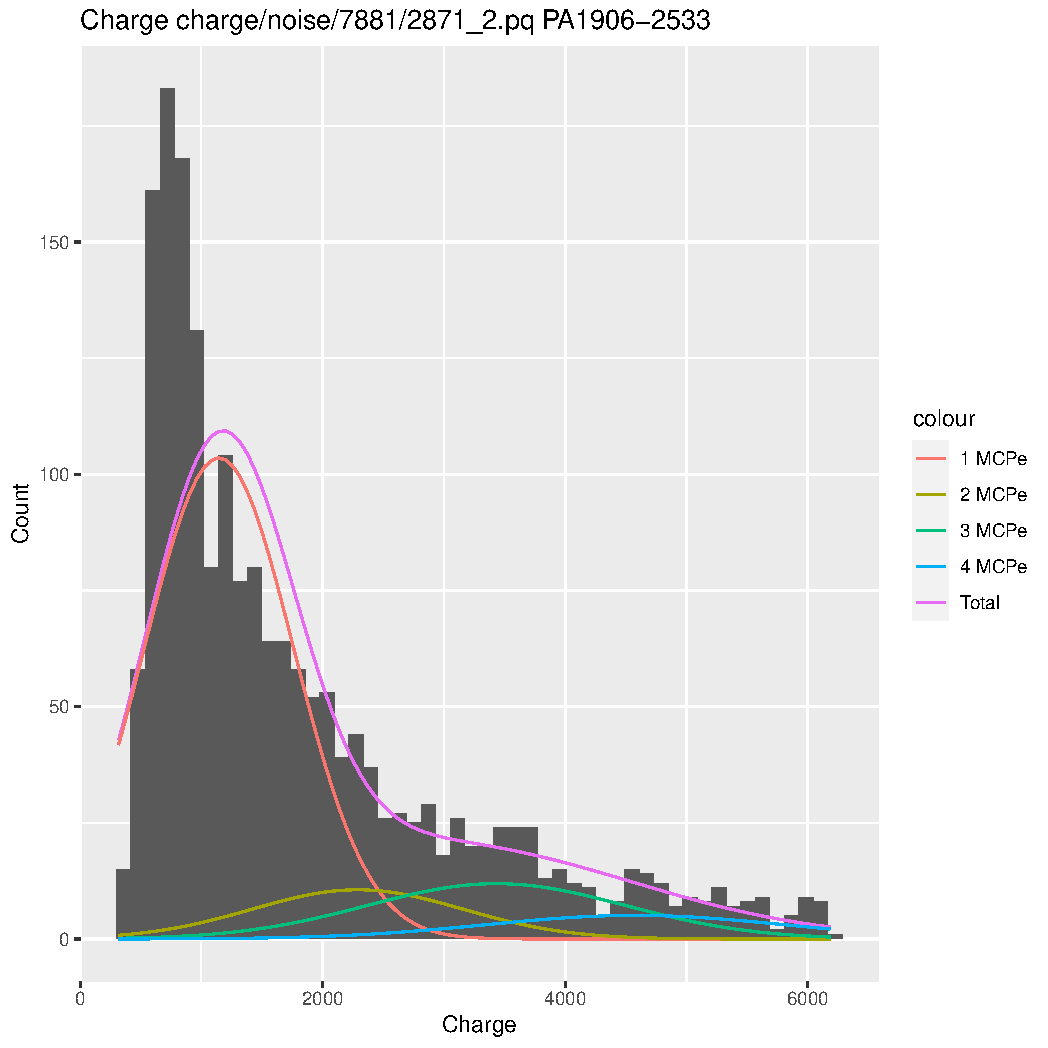
\includegraphics[width=0.6\textwidth]{charge_7881_2871_2_gaussian.pdf}
    \caption{Gaussian Mixture Model Fit}
    \label{fig:gauss-mixture}
\end{figure}

\subsection{Gamma Tweedie Mixture Model}
Jun Weng proposed a charge model based on MCP and ALD mechanism, suggesting that
the number of true-secondary electrons follows Poisson distribution, 
and single electron charge response follows Gamma distribution.
Therefore, the total charge response could be considered as a mixture of
Gamma and compound Poisson-Gamma distributions\cite{wengSingleElectronCharge2024}:
\begin{equation}\label{eq:mixture}
    \begin{aligned}
        Q_{\mathrm{MCP-PMT}}& =p_{0}\times Q_{\mathrm{peak}}+(1-p_{0})Q_{\mathrm{ts}} \\
        &=p_{0}\times Q_{\mathrm{peak}}+(1-p_{0})\sum_{n=0}^{\infty}\sum_{i=0}^{n}Q_{\mathrm{i}}
    \end{aligned}
\end{equation}

In equation~\ref{eq:mixture}, $p_{0}$ is the probability of PE not emitting secondary electrons,
$Q_{\mathrm{peak}}$ and $Q_{i}$ follow Gamma distribution, 
and the number of true-secondary electrons $n$ follows Poisson distribution.

Especially, compound Poisson-Gamma distribution is a special case of Tweedie distribution,
whose power parameter statisfies $p\in(1, 2)$.
Tweedie distribution is widely used in generalized linear regression.

\section{Mixture Fit Methods}
\subsection{Non-linear Least Square Methods}
Assume the the parameters are $\theta=\left(\alpha, \beta, \mu, \phi, p\right)$, 
observed charge data set is $\left(y_{1},y_2,\cdots,y_n\right)$, 
and the mixture distribution function is $f(y)=\pi f_{1}(y)+(1-\pi)f_{2}(y)$. 
The target parameters are:
\begin{equation} 
    \psi_{\text{LS}}=\operatorname*{argmin}_{\left(\theta,\pi\right)} 
    \sum\limits_{i}\left[\left(y_i-f(y|\theta)\right)^{2}\right]
\end{equation}

Then $\mu_{q}, \sigma_{q}^{2}$ are:
\begin{equation}
    \begin{aligned}
    \mu_{q} & = \pi\cdot\frac{\alpha}{\beta}+(1-\pi)\cdot\mu\\
    \sigma_{q}^2 & = \pi^2\cdot\frac{\alpha}{\beta^2}+(1-\pi)^2\cdot\mu^p\phi
    \end{aligned}
\end{equation}

\subsection{Expectation Maximization Algorithm}
At the $(r+1)$ iteration, the posterior probability of $y_{i}$ belonging to $k$ th mixture component is:
\begin{equation}
    \hat{p}_{ik}^{(r+1)}=\frac{\hat{\pi}_k^{(r)}f_k(y_i\mid\hat{\theta}_k^{(r)})}
    {\sum_{h=1}^{\mathcal{K}}\hat{\pi}_h^{(r)}f_h(y_i\mid\hat{\theta}_h^{(r)})}\enspace(k=1,2)
\end{equation}

Q function is defined as the expectation of log-likelihood (E-step):
\begin{equation}
    Q=\sum_{k=1}^{2}\sum_{i=1}^{n}\hat{p}_{ik}^{(r+1)}\log f_{k}(y_{i})+\sum_{k=1}^{2}\sum_{i=1}^{n}\hat{p}_{ik}^{(r+1)}\log\pi_{k}
\end{equation}

Gamma distribution $f_{1}(y)$ and Tweedie distribution $f_{2}(y)$ is irrelevant, therefore could be maximized separately.

Use $\hat{\theta}_{k}^{(r)},\hat{\pi}_{k}^{(r)}$ to generate new parameters (M-step):
\begin{equation}
    \begin{aligned}
        \hat{\theta}_{k}^{(r+1)}&=\operatorname*{argmax}_{\theta} \sum_{i=1}^{n}\hat{p}_{ik}^{(r+1)}\log f_{k}(y_{i})\\
        \hat{\pi}_{k}^{(r+1)}&=\frac1n\sum_{i=1}^n\hat{p}_{ik}^{(r+1)}
    \end{aligned}
\end{equation}

$\hat{\theta}^{(\infty)}, \hat{\pi}^{(\infty)}$ 
are the final estimated posterior parameters and mixture ratio.

\subsection{Correlation}
If the charge model is accurate, meaning residuals $y_{i}-f(y)\stackrel{\text{i.i.d}}{\sim}N(\mu, \sigma^{2})$,
NLS is exactly the same as EM:
\begin{equation}
\ell(\theta)=\sum_i\log P(y_i|\theta)=-\frac{1}{2\sigma^{2}}\sum_{i}(y_{i}-f(y))^{2}
-n\log\sigma-\frac{n}{2}\log2\pi
\end{equation}

% 默认使用正文的参考文献样式;
% 如果使用 BibTeX,可以切换为其他兼容 natbib 的 BibTeX 样式。
\bibliographystyle{unsrtnat}
% \bibliographystyle{IEEEtranN}

% 默认使用正文的参考文献 .bib 数据库;
% 如果使用 BibTeX,可以改为指定数据库,如 \bibliography{ref/refs}。
\printbibliography

\end{survey}
